\documentclass[tikz,border=10pt]{standalone}
\begin{document}
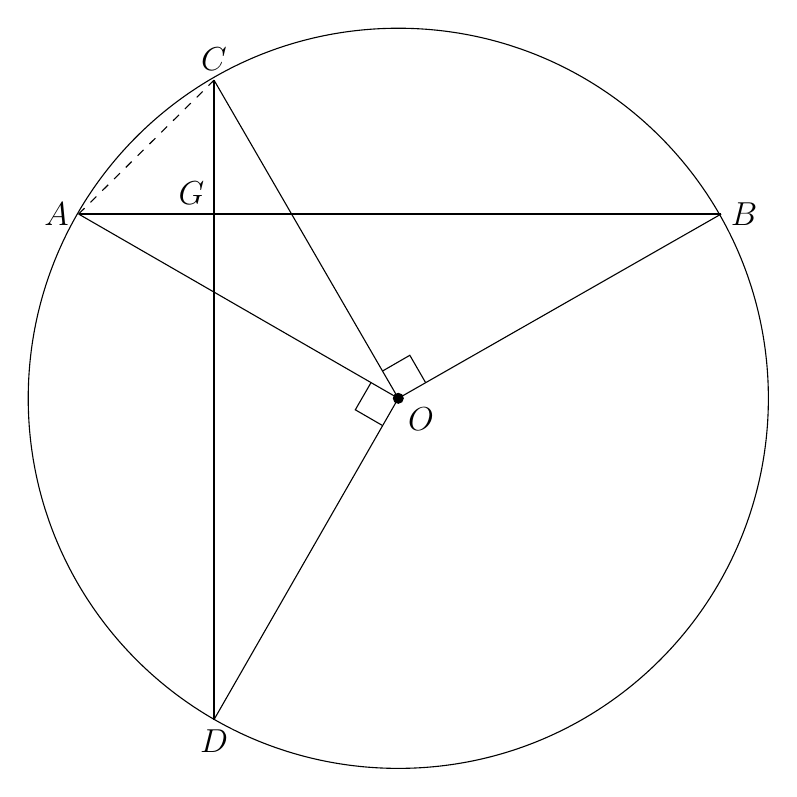
\begin{tikzpicture}[scale=1, every node/.style={font=\large}]
\coordinate (O) at (0,0);
\coordinate (C) at (-2.34,4.04);
\coordinate (A) at (-4.06,2.34);
\coordinate (B) at (4.10,2.34);
\coordinate (D) at (-2.34,-4.08);
\coordinate (G) at (-2.34,2.34);

\draw (O) circle (4.7);

\draw (A) -- (B);
\draw (C) -- (D);
\draw[dashed] (A) -- (C);
\draw (A) -- (O);
\draw (C) -- (O);
\draw (B) -- (O);
\draw (D) -- (O);

\draw (0.4*-0.5,0.4*0.866) -- (0.4*-0.5+0.4*0.866,0.4*0.866+0.4*0.5) -- (0.4*0.866,0.4*0.5);
\draw (-0.346,0.2) -- (-0.546,-0.146) -- (-0.2,-0.346);

\fill (O) circle (2pt);

\node[above] at (C) {$C$};
\node[left] at (A) {$A$};
\node[right] at (B) {$B$};
\node[below] at (D) {$D$};
\node[above left] at (G) {$G$};
\node[below right] at (O) {$O$};
\end{tikzpicture}
\end{document}
